% !TeX encoding = UTF-8
% !TeX spellcheck = it_IT
% !TeX root = MatDiz.tex
\chapter{E}
\vspace{5mm} 
\lemma{e} Costante numerica. $e$ numero irrazionale \pointsto~\seeentry{n. irrazionale} trascendente \pointsto~\seeentry{n. trascendente}. Nel 1728 Euler lo usa come base dei logaritmi naturali.
\lemma{Euclide}\index{Euclide}
\lemma{Euler Leonard}\index{Euler Leonard}(1707-1783) Nato vicino a Basilea. Fu allievo di Johann I Bernulli\pointsto~\vedilemma{Bernoulli Johann}\index{Bernulli Johann} trasferitosi all'accademia di S.Pietroburgo li divenne assistente di Daniel Bernulli \pointsto~\vedilemma{Bernoulli Daniel}\index{Bernulli Daniel} per poi succedergli. La sua produzione è sterminata in tutti i campi della matematica ed oltre. Il 7 settembre 1783 secondo le parole del marchese di Condorcet, <<cesso di calcolare e di vivere>>. 
\begin{figure}
	\centering
	\scaptionb{Leonhard Euler (1707-1783)}
	\label{fig:leonhardeuler}
	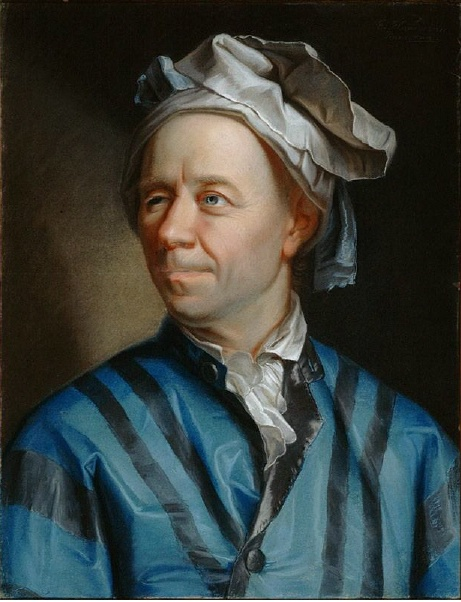
\includegraphics[width=0.7\linewidth]{Figure/E/Leonhard_Euler}
	\floatfoot{\selectlanguage{english}{Di Jakob Emanuel Handmann - 2. Kunstmuseum Basel1. digitized version, the source (scanner) of the digitized image is unknown.The image was transferred from en.wiki (en:Image:Leonhard Euler.jpg) under the {{PD-old}} license tag. Wars 16:56, 25 June 2006 (UTC), Pubblico dominio,} \url{https://commons.wikimedia.org/w/index.php?curid=893656}}
\end{figure}
